%%%%%%%%%%%%%%%%%%%%%%%%%%%%%%%%%%%%%%%%%%%%%%%%%%%%%%%%%%%%%%%%%%%%%%%%%%%%%%%%
%2345678901234567890123456789012345678901234567890123456789012345678901234567890
%        1         2         3         4         5         6         7         8

\documentclass[letterpaper, 10 pt, conference]{ieeeconf}  % Comment this line out if you need a4paper

%\documentclass[a4paper, 10pt, conference]{ieeeconf}      % Use this line for a4 paper

\IEEEoverridecommandlockouts                              % This command is only needed if 
                                                          % you want to use the \thanks command

\overrideIEEEmargins                                      % Needed to meet printer requirements.

% See the \addtolength command later in the file to balance the column lengths
% on the last page of the document

% The following packages can be found on http:\\www.ctan.org
\usepackage{graphicx} % for pdf, bitmapped graphics files
%\usepackage{epsfig} % for postscript graphics files
%\usepackage{mathptmx} % assumes new font selection scheme installed
%\usepackage{times} % assumes new font selection scheme installed
\usepackage{amsmath} % assumes amsmath package installed
\usepackage{amssymb}  % assumes amsmath package installed

\title{\LARGE \bf
Return Oriented Programming on an Embedded System Using Code Injection
}


\author{Justin Cox and Tyler Travis
\\ \small{Deptartment of Electrical and Computer Engineering}
\\ \small{Utah State University}
\\ \small{Logan, Utah 84322}
\\ \small{email: justin.n.cox@gmail.com, tyler.travis@aggiemail.usu.edu}
}

\usepackage{listings}
\usepackage{color}

\definecolor{dkgreen}{rgb}{0,0.6,0}
\definecolor{gray}{rgb}{0.5,0.5,0.5}
\definecolor{mauve}{rgb}{0.58,0,0.82}

\lstset{frame=none,
  language=C,
  aboveskip=3mm,
  belowskip=3mm,
  showstringspaces=false,
  columns=flexible,
  basicstyle={\small\ttfamily},
  numbers=none,
  numberstyle=\tiny\color{gray},
  keywordstyle=\color{blue},
  commentstyle=\color{dkgreen},
  stringstyle=\color{mauve},
  breaklines=true,
  breakatwhitespace=true,
  tabsize=3
}

\begin{document}



\maketitle
\thispagestyle{empty}
\pagestyle{empty}


%%%%%%%%%%%%%%%%%%%%%%%%%%%%%%%%%%%%%%%%%%%%%%%%%%%%%%%%%%%%%%%%%%%%%%%%%%%%%%%%
\begin{abstract}

This paper describes the process of implementing a code injection attack on an ARM Cortex M4 through Return Oriented Programming.  The paper will describe the process of selecting useful snippets of code found in the ROM of a microcontroller.  The paper will end by showing the injected program working on the microcontroller.  

\emph{Index Terms}---Return Oriented Programming (ROP), stack overflow, security, embedded system, canary.    

\end{abstract}

%%%%%%%%%%%%%%%%%%%%%%%%%%%%%%%%%%%%%%%%%%%%%%%%%%%%%%%%%%%%%%%%%%%%%%%%%%%%%%%%
\section{INTRODUCTION}

Every year, the amount of devices with embedded systems greatly increases.  With the demand that every device connect to the internet (Internet of Things), in the near future almost all devices will have an embedded system.  That being said, generally these embedded devices are not manufactured with security as the top priority.

Buffer overflow attacks have been widely demonstrated and used to allow a hacker to gain control over a system or program.  Most of the buffer overflow techniques on x86-64 architectures have been well researched and defended against.  However, this is not the case for embedded systems.  Using more advanced buffer overflow techniques such as Return Oriented Programming (ROP), an attacker is able to utilize the manufacture's driver libraries and boot code found on the ROM to take over an embedded device.  This vulnerability will become more threatening when most common, household items have embedded devices such as microcontrollers.       

%\begin{figure}[thpb]
%	\centering
%	\includegraphics[scale=0.5]{sha1}
%    \caption{A flowchart of one iteration within the SHA1 compression %function where blocks $A,B,C,$ and $D$ are 32-bit words.}
%\end{figure}
 

\section{VULNERABILITY OVERVIEW}
     

\subsection{Overview of ROP}

As stack based, buffer overflow attacks became more common, programmers and researchers came up with methods to defend against these attacks.  A simple method of defense is to prohibit a section of memory to be both wrote to and executed from.  If an attacker was able to accomplish a buffer overflow, the attacker would not be able to return and execute the malicious code on the stack.  In response to this defense, attackers came up with ways to use the code already found on most systems, e.g. libraries such as libc.  One of these more advanced methods of attack is Return Oriented Programming (ROP).

ROP allows the attacker to gain control flow over a program by using useful snippets of code found in drivers and/or libraries called "gadgets".  After execution, each gadget needs to end with a return command.  The return command allows the attacker to return to another gadget or eventually to a malicious program.

In the case of an ARM architecture, there are no "return" commands so branches and pop instructions can be used instead to achieve the same result [1].  

\subsection{Buffer Overflow}

The vulnerable function that will be exploited to allow a buffer overflow is the following:

\begin{lstlisting}
void echo(void){
	
	char buffer[32];
	
	UARTgets(buffer, sizeof(buffer));
	
	UARTprintf("%s \n", buffer);
	
}
\end{lstlisting}

\noindent
The UARTgets() and UARTprintf() functions are provided from the TivaWare libraries from TI.  In order to be able to overflow the character buffer of size 32, we had to remove the bounds checking done in the UARTgets() function.  It is worth noting that for certain user-input obtaining functions, the function stops getting the input when it encounters the null character $0$x$00$.  This is not the case for UARTgets(), making the ROP attack easier to develop.  The malicious code will be inserted onto the stack as the character buffer is overflowed.

\subsection{Overcoming Canary Stack Protection}

Another defense used to stop buffer overflow attacks is the use of a canary.  The main objective of a buffer overflow is to overwrite the functions return address.  A canary is placed in between the buffer and the return address.  Before the program returns from the return address, it checks to see if the canary has been modified.  If it has, it throws an exception and program execution is halted.

The IDE being used to program the echo() program onto the microcontroller is Keil uVision.  In Keil, there are options available to turn on stack protection.  For stack protection in Keil, the canaries are defined by the programmers.  A randomly generated canary is the best choice for increased security.  However since the generation of random canaries takes a toll on the overall performance of the microcontroller, often times a static canary is used.  A common canary that is used is a 32-bit word containing nulls, e.g. $0$x$00000000$ [2].  The authors chose to use the null canary and a later section in this paper will explain how the canary was overcome. 
%\begin{figure}[thpb]
%	\centering
%	\includegraphics[scale=.75]{passwordGeneration}
%    \caption{An example table that shows how the password generation %must generate passwords.}
%\end{figure}

%$$w[16] = w^{'}[16]\ XOR\ w[0]\_1$$
%$$w[17] = w^{'}[17]$$
%$$w[18] = w^{'}[18]$$
%$$w[19] = w^{'}[19]\ XOR\ w[0]\_2$$

%\noindent

%\begin{center}
%    \begin{tabular}{| p{4cm} | l |}
%        \hline
%         Optimization & Million Hashes per Second \\ \hline
%        Baseline (AVX + Loop Unrolling) & .73 \\ \hline
%        Optimization 1 (Baseline + XOR exploit) & 3.45 \\ \hline
%        Optimization 2 (Baseline + pthreads) & .80 \\ \hline
%        Combined Optimization & .87 \\
%        \hline
%    \end{tabular}
%\end{center}


\section{CODE INJECTION}

In order to inject the attackers code, the microcontroller's flash memory needs to be erased and then reprogrammed.  The microcontroller that will be used is the TM4C123G, more specifically, the Tiva C LaunchPad from Texas Instruments.  The TM4C123G has a ARM Cortex M4 architecture that uses the Thumb-2 instruction set.

In order to erase the flash, the following must be performed:

\begin{enumerate}
\item Write the flash key and MERASE bit to the FMC register
\item Wait for flash erase routine to finish
\end{enumerate}

In order to reprogram the flash, the following must be performed:

\begin{enumerate}
\item Write data to the FWBn registers
\item Write the start address of program into the FMA register
\item Write the flash key and WRBUF bit to the FMC2 register
\item Wait for flash write routine to finish
\end{enumerate}

In order to accomplish the above procedures, the ROP gadgets will need to be able to perform loads from the stack as well as perform a store to a desired memory location.

A program was written in C++ to send the malicious data over a COM port that interfaces with a UART module on the microcontroller.

\section{GADGET SELECTION}

There is one function that is needed to erase the flash, write to the flash buffer, and commit the flash write buffer into the flash memory. That function needs to write certain data to an in-memory register. This overall fuction is broken down into 3 subsections:

\begin{enumerate}
\item Load the correct data off of the stack into a register
\item Load the correct address off of the stack into a register
\item Store the data into the address
\end{enumerate}

Gadget one through three correspond to the list above. 

Gadget one:
\begin{lstlisting}
    ldr r0, [r4, #4]
    pop {r4, pc}
\end{lstlisting}

Gadget two:
\begin{lstlisting}
    pop {r4, pc}
\end{lstlisting}

Gadget three:
\begin{lstlisting}
    str r0, [r4, #0]
    pop {r4, pc}
\end{lstlisting}

Gadget four is used for a delay when the flash is getting erased or written to
\\
\\
Gadget four:

\begin{lstlisting}
    tst.w r0, #8
    ite ne
    movne #15
    moveq #14
    pop {pc}
\end{lstlisting}

The actual instruction functionality of gadget four isn't important, only the amount of time it takes to execute.

\section{IMPLEMENTATION}

Using the gadgets explained in the previous section, a carefully crafted byte string was sent over UART into the character buffer on the microcontroller.  Assuming the attacker has the ability to attempt the buffer overflow many times, the canary value was discovered to be a 32-bit word of null characters.  This null canary was precisely placed in the byte string to preserve the canary.

Following the canary, the initial gadget was placed in the spot of the former return address.  This initial portion of the attack byte string is illustrated in Figure 1.

\begin{figure}[thpb]
	\centering
	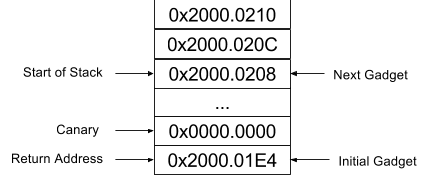
\includegraphics[scale=.50]{TheInitialStack}
    \caption{An example of how the buffer overflow attack is initialized.}
\end{figure}

The next part of the attack string handles the flash memory erase routine.  The section of stack memory pertaining to the flash erase routine is further explained in Figure 2.  

\begin{figure}[thpb]
	\centering
	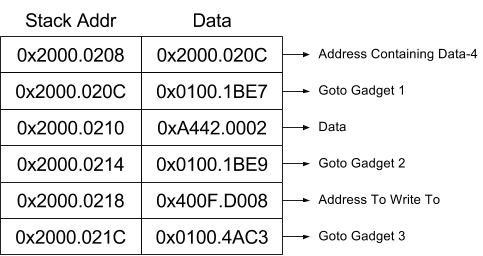
\includegraphics[scale=.50]{RegisterWriting}
    \caption{An example of how the gadgets are stored on the stack to perform multiple load and stores.}
\end{figure}

After the flash erase routine is performed, the attack byte string has a large number of delay gadgets to allow the erase to finish.  A large amount of delay gadgets are also used when the flash write routine is performed.

The next part of the attack string is used to load the new program data into the flash memory write-data buffers.  This routine is repeated for all of the opcodes that need to be loaded.

The last portion of the attack sets the PC address to the beginning address of the newly loaded program.  The program will begin without having to restart the microcontroller.  This feature allows an attacker to inject the malicious code remotely.    
%	\centering
%	\includegraphics[scale=.35]{tek00001}
%    \caption{The blue signal is when the program initiates. The %yellow signal is when the hash has been computed and verified.}
%\end{figure} 

\section{RESULTS}

The authors were able to successfully perform a code injection attack using ROP.  The microcontroller was initially programmed to perform an "echo" functionality.  Using a buffer overflow with ROP, the authors were able to erase the flash, reprogram the flash, and start the new program.  The new program flashes an LED found on the Tiva C Launchpad at a human observable rate.  Here is a picture of the successful hack.

\begin{figure}[thpb]
	\centering
	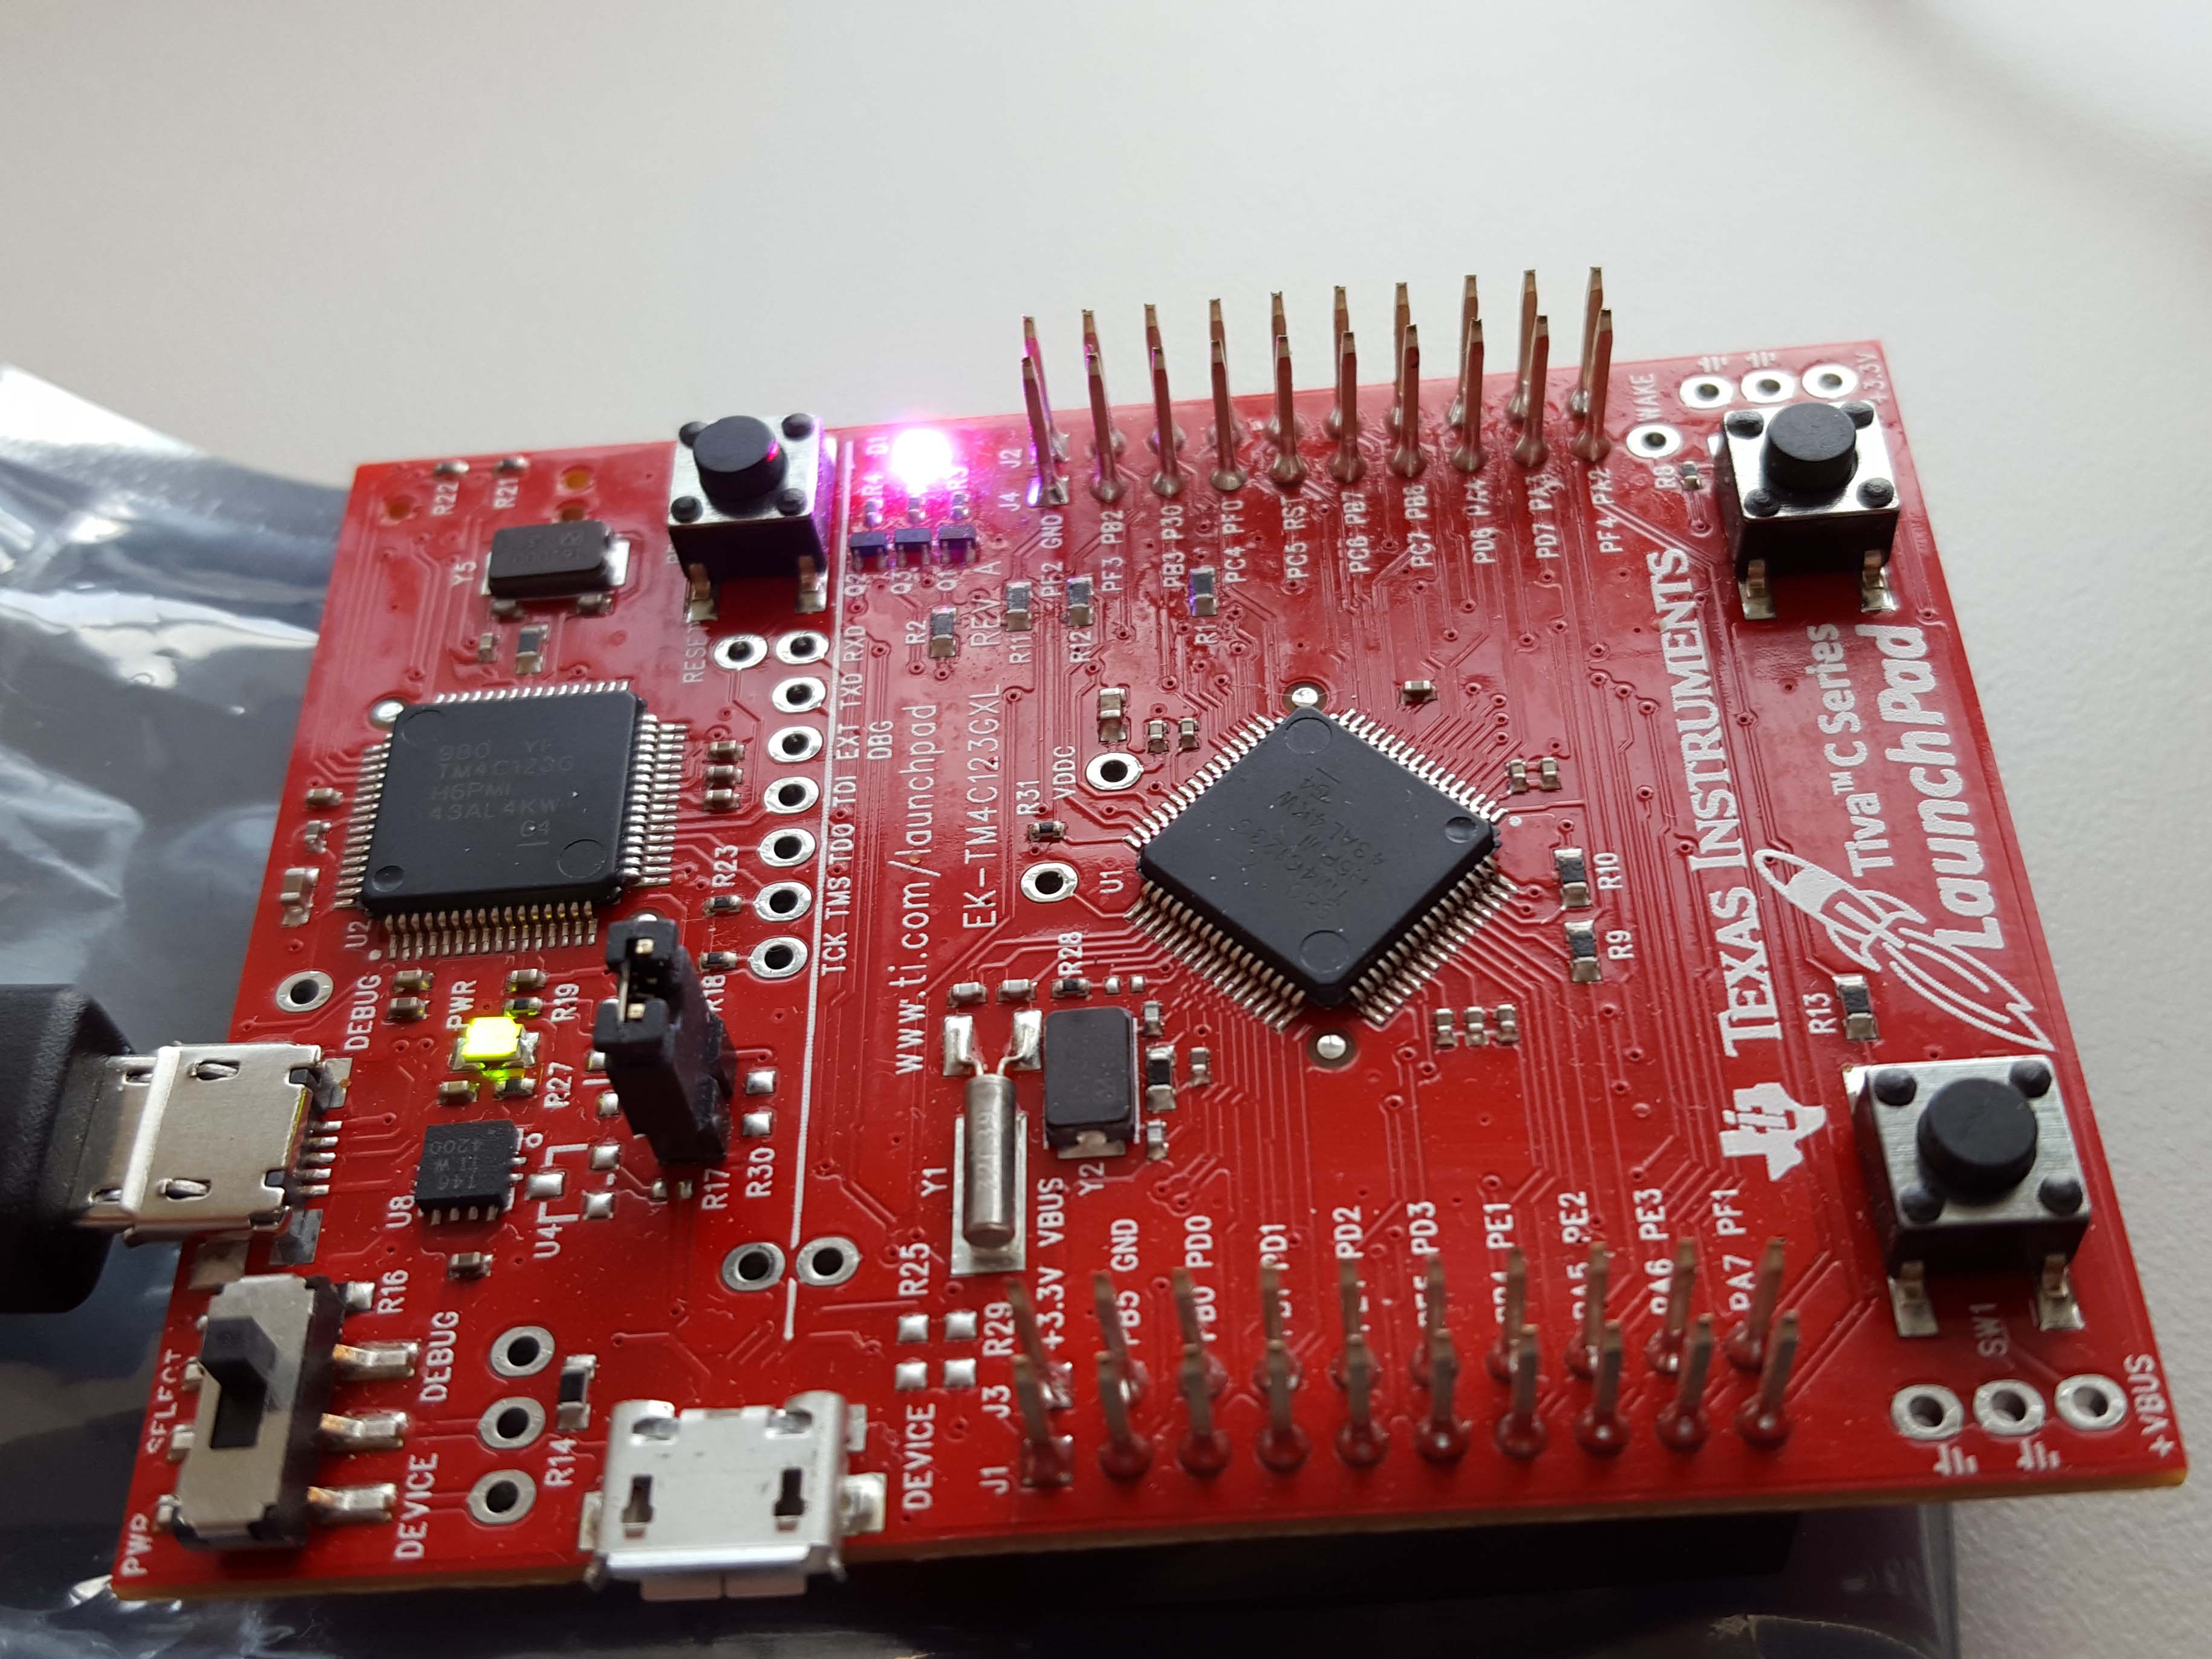
\includegraphics[scale=.05]{board}
    \caption{Successful code injection of a blinky program.}
\end{figure}
  
\subsection{Problems Encountered}

The flash erase and flash write routines require a delay time.  In order to satisfy the delay time, many delay gadgets were used to "waste time".  It would be better to find a gadget that is able to poll the READY bit.  This is something that can be enhanced in a future implementation.  It would allow the attack byte string to be much smaller.

\section{CONCLUSION}

This attack proves that code can be injected onto the TM4C123G microcontroller. Given the right circumstances, code can be erased and executed by exploiting the internal ROM by using ROP on an ARM device. This implies that all TM4C123G microcontroller of this family are vulnerable to this type of attack. Microcontrollers and embedded systems need to achieve better security to keep up with newer attacks to their systems.

\addtolength{\textheight}{-12cm}   % This command serves to balance the column lengths
                                  % on the last page of the document manually. It shortens
                                  % the textheight of the last page by a suitable amount.
                                  % This command does not take effect until the next page
                                  % so it should come on the page before the last. Make
                                  % sure that you do not shorten the textheight too much.

%%%%%%%%%%%%%%%%%%%%%%%%%%%%%%%%%%%%%%%%%%%%%%%%%%%%%%%%%%%%%%%%%%%%%%%%%%%%%%%%



%%%%%%%%%%%%%%%%%%%%%%%%%%%%%%%%%%%%%%%%%%%%%%%%%%%%%%%%%%%%%%%%%%%%%%%%%%%%%%%%



%%%%%%%%%%%%%%%%%%%%%%%%%%%%%%%%%%%%%%%%%%%%%%%%%%%%%%%%%%%%%%%%%%%%%%%%%%%%%%%%

%\section*{ACKNOWLEDGMENT}

%The author would like to thank his instructor Dr. Rajnikant Sharma %for his help in understanding control concepts.




%%%%%%%%%%%%%%%%%%%%%%%%%%%%%%%%%%%%%%%%%%%%%%%%%%%%%%%%%%%%%%%%%%%%%%%%%%%%%%%%




\begin{thebibliography}{99}

\bibitem{c1} L. Davi, A. Dmitrienko, A. R. Sadeghi, M. Winandy, "Return-Oriented Programming without Returns on ARM," System Security Lab, Ruhr University Bochum, Germany, Tech. Rep. HGI-TR-2010-002, July 2010.
\bibitem{c2} G. Richarte, "Four different tricks to bypass StackShield and StackGuard protection," Core Security Technologies, April 2002.
 

\end{thebibliography}

\begin{figure}[thpb]
	\centering
	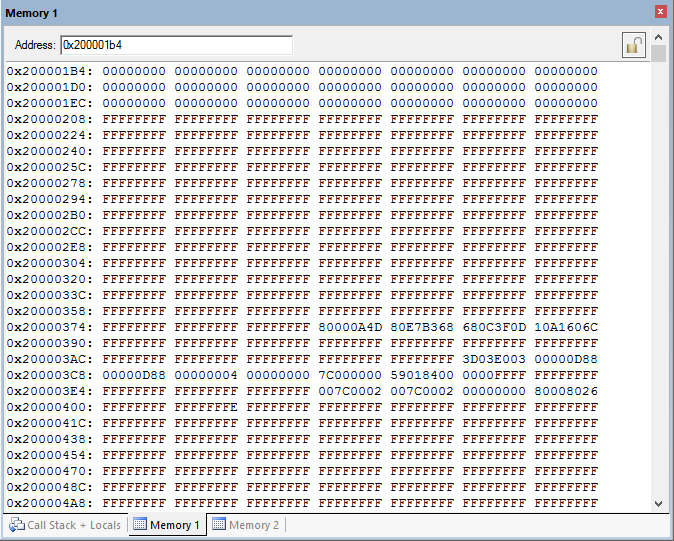
\includegraphics[scale=.5]{StackB4}
    \caption{The stack memory before the attack.}
\end{figure}

\begin{figure}[thpb]
	\centering
	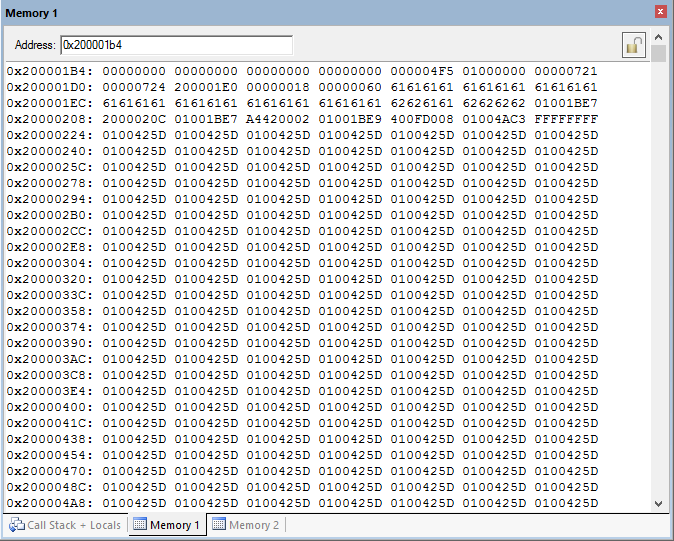
\includegraphics[scale=.5]{Stack_After1}
    \caption{A beginning portion of the stack memory after the attack.}
\end{figure}

\begin{figure}[thpb]
	\centering
	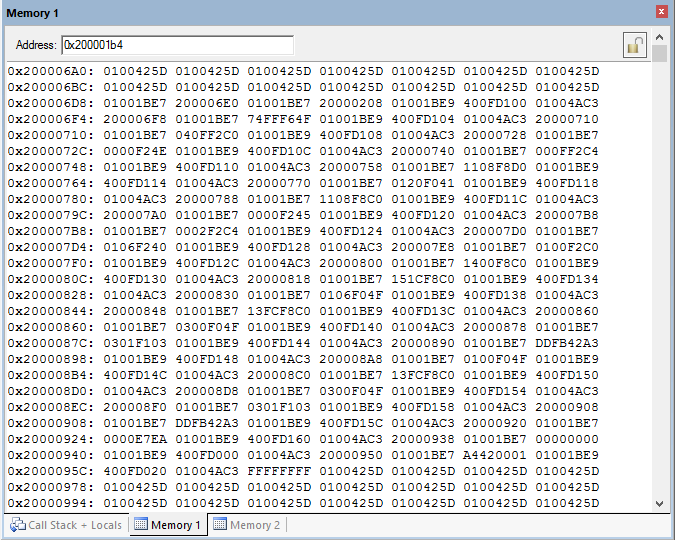
\includegraphics[scale=.5]{Stack_After2}
    \caption{A portion of the stack memory with the opcodes after the attack.}
\end{figure}


\end{document}
